\documentclass[11pt]{article}
\usepackage{calc}
\usepackage{color}
\usepackage{amsfonts}
\usepackage{latexsym}
\usepackage{placeins}
\usepackage[a4paper,top=5.5cm,bottom=4cm,left=2.5cm, right=2.5cm,foot=1cm]{geometry}
\pagenumbering{gobble}
\usepackage{setspace,relsize}               
\usepackage{moreverb}                        
\usepackage{url}
\usepackage{hyperref}
\hypersetup{colorlinks=true,citecolor=blue}
\usepackage{mathtools} 
\usepackage{amsthm}
\usepackage{amssymb}
\usepackage{indentfirst}
\usepackage{todonotes}
\usepackage{subfigure}
\usepackage[numbers,square]{natbib}
\bibliographystyle{plain}
\usepackage[pdftex]{lscape}
\usepackage{authblk}
\usepackage{amsmath}
\usepackage[cp1250]{inputenc}
\usepackage[OT4]{fontenc}

\addtolength{\voffset}{-3.5cm} \addtolength{\textheight}{4cm}

\renewcommand{\refname}{\large{\textbf{ Bibliography}}}
\renewcommand\Authfont{\scshape\small}
\renewcommand\Affilfont{\itshape\small}
\newcommand{\keywords}[1]{\noindent{\large{\bf Keywords:}} #1\\}
\setlength{\affilsep}{1em}
\newcommand{\smalllineskip}{\baselineskip=15pt}
\newcommand{\emailaddress}[1]{{\sf#1}}
\newcommand{\speaker}[1]{\author{\underline{#1}}}
\newcommand{\speakeraffil}[1]{\affil{#1}}
\let\LaTeXtitle\title
\renewcommand{\title}[1]{\LaTeXtitle{\Large{\textbf{#1}}}}

% Title Page
\title{Some remarks on the uncertainty analysis of $R_0$ in the SIR model}

\speaker{Luiz Max F. de Carvalho} % Write speaker name here

\author[1]{Daniel A. M. Villela}
\author[2]{Flavio Coelho}
\author[1]{Leonardo S. Bastos}

%%AFFILIATIONS
\speakeraffil{Program for Scientific Computing (PROCC), Oswaldo Cruz Foundation, Brazil,\,\emailaddress{lmax.procc@gmail.com}} % Write affiliation/s of the speaker here.
\affil[2]{School of Applied Mathematics, Getulio Vargas Foundation (FGV), Brazil,\,\emailaddress{fccoelho@fgv.br}} % Write affiliation/s of the first co-author here, if there is any. If not, remove the line.

\date{\vspace{-6ex}} % Do not modify this line

\DeclareMathOperator*{\argmin}{arg\,min}
\DeclareMathOperator*{\argmax}{arg\,max}
\newtheorem{theo}{Theorem}[]
\newtheorem{proposition}{Proposition}[]
\newtheorem{remark}{Remark}[]
\setcounter{theo}{0} % assign desired value to theorem counter
\begin{document}

\maketitle

\keywords{Basic reproductive number; uncertainty; logarithmic pooling; Gamma ratio distribution.}

The basic reproductive number, $R_0$, is a key quantity in epidemic modelling and defines the threshold of disease-free equilibrium for many deterministic models of disease.
It is usually a quantity of interest when constructing mathematical models of infectious diseases and developing and evaluating mitigation strategies.
While most well studied mathematical models are deterministic in nature, acknowledging uncertainty on parameter values is important because predictions can be sensitive to changes in parameter values.
In addition, most interesting models are nonlinear which makes correlations between parameters difficult to study analytically.

A seminal paper by Poole~\& Raftery~\cite{poole2000} discusses the issue of propagating uncertainty through a deterministic model.
The authors use an operator called the logarithmic pooling (LP) operator to combine prior distributions induced by the structure of the model.
The operator takes a set of probability distributions $F(\boldsymbol\theta)$ and a set of weights $\boldsymbol\alpha$ and combines them into a single probability distribution $\pi(\boldsymbol\theta)$.

Here we are concerned with the following setting: suppose $K$ experts express their opinions on a parameter $\boldsymbol\theta \in \Theta \subseteq \mathbb{R}^{p}$ by means of a set of (proper) probability distributions $F(\boldsymbol\theta) = \{ f_1(\boldsymbol\theta), f_2(\boldsymbol\theta), \ldots, f_K(\boldsymbol\theta) \}$.
Supposed further that we are also interested in a quantity $\mathbf{y} \in  \mathcal{Y}  \subseteq \mathbb{R}^{q}$ that relates to $\boldsymbol\theta $ through a deterministic model $M(\boldsymbol\theta) = \mathbf{y}$.
We would like to obtain one distribution on $\mathbf{y}$ to represent our uncertainty about this quantity \textit{induced} by the uncertainty we have on $\boldsymbol\theta$.
This, however, begs the question of in which order the pooling and propagation (or inducing) operations should be performed.
One could either (a) compute the induced distributions for each expert and then combine these using LP or (b) combine the distributions first and then apply $M(\cdot)$ to obtain a distribution on $\mathbf{y}$.

While it is relatively straightforward to show that procedures (a) and (b) will yield the same distribution if $M(\cdot)$ is invertible, the question remains open for the case of non-invertible models, which correspond to the vast majority of epidemic models.

In this paper we study the uncertainty analysis for $R_0$ in the constant population 	Susceptible-infectious-Removed (SIR) model.
We show that if uncertainty about the transmission rate $\beta$ and recovery rate $\gamma$ can be expressed using Gamma distributions, the induced distribution on $R_0$ has a closed-form solution which is a variant of the generalised Beta prime distribution.
This distribution, henceforth called Gamma ratio (GR) distribution has been derived in a more general setting by Coelho \& Mexia~\cite{Coelho2007} and is sub-exponential, being log-concave only on an interval that depends on its four parameters.%%, which we provide.

We explore the case when one has a set of distributions on both $\beta$ and $\gamma$ and desires to obtain a distribution on $R_0$.
This model is non-invertible, since, for a population of size $N$,  $R_0 = \beta N/\gamma$.
Thus, the distributions on $R_0$ obtained using procedures (a) and (b) need not coincide. % LM: Clearly, (a) and (b) only lead to the same distribution in the trivial case $\alpha_j = 1$, which is a danger for the KL approach.
We show that they indeed yield different distributions.
While procedure (a) induces a reasonably well-behaved GR distribution, procedure (b) leads to a distribution with heavier tails and for which closed-form solutions are available only under some restrictions on the original distributions on the parameters.
A in-depth analysis of tail behaviour and some general guarantees are provided for both distributions, focusing on the comparison the two.
We consider this comparison to be key in understanding how to best deal with the order of pooling and inducing operations in non-invertible models.

A way to reconcile these two distributions could be to choose the vector of weights $\boldsymbol\alpha$ for LP such that the Kullback-Leibler (KL) divergence between the two is minimised.
This approach attempts to assign each expert a weight in order to combine distributions on $\boldsymbol\theta$ whilst minimising divergence in transformed space.
Since usually distributions for $\boldsymbol\theta$ are not elicited with $\mathbf{y}$ in mind, this approach takes advantage of the discrepancy that arises for non-invertible models to assign the weights in a principled manner, as opposed to arbitrarily giving each expert/information source a weight.

In Figure~\ref{fig:abstractFigure} we show the ``induce-then-pool'' and ``pool-then-induce'' distributions obtained for $R_0$ using four simulated pairs of distributions (panel A) and also the resulting distribution for $R_0$ using the KL divergence minimisation procedure sketched above (panel B).

\section*{Acknowledgements}
[PUT YOURS IN, BOYZ]
\bibliography{R0}

% \begin{figure}[!ht]
% \centering
% \includegraphics[width=\textwidth, height = 15cm]{figures/}
% \caption{\textbf{}.
% }
% \label{fig:}
% \end{figure}
% %
\begin{figure}
\hfill
\subfigure[A]{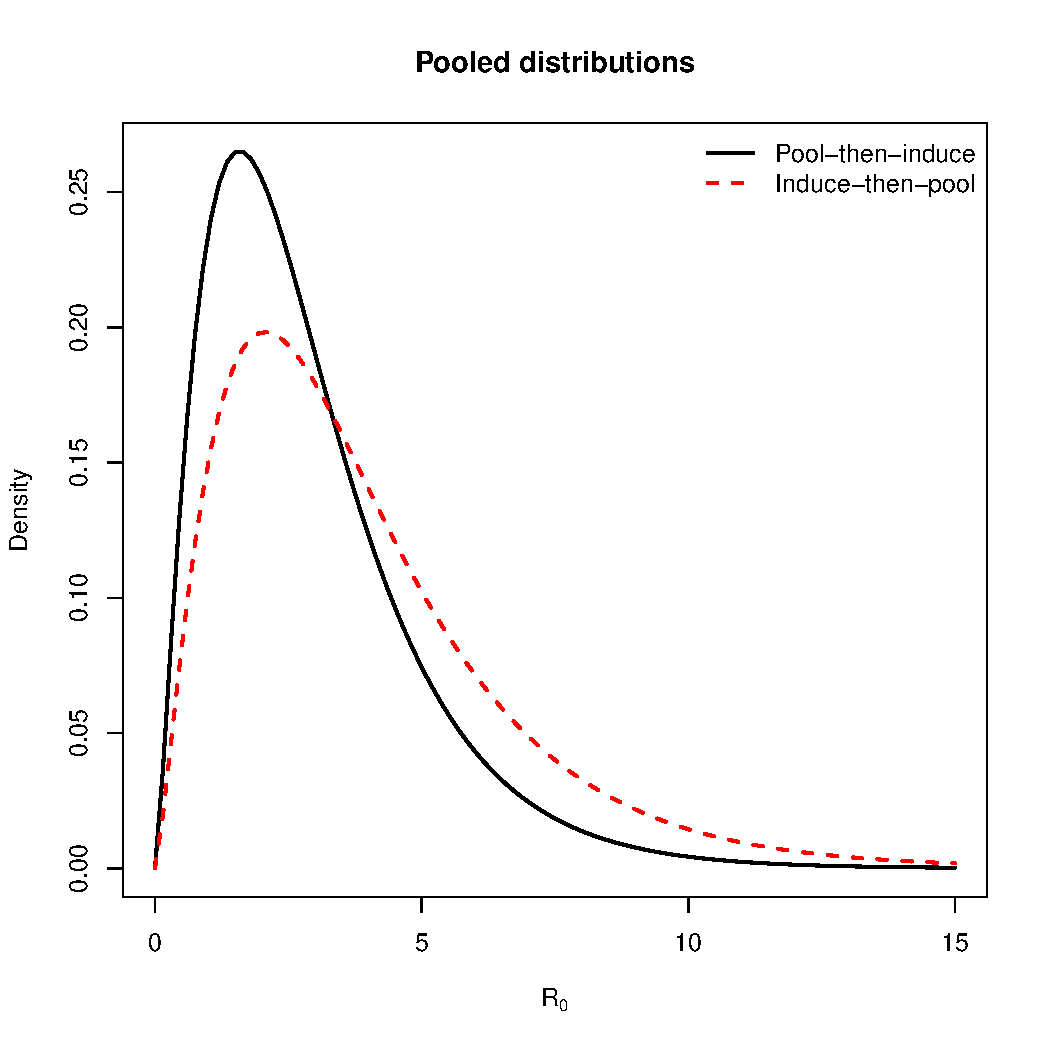
\includegraphics[scale=0.35]{figures/ItP_vs_PtI_equalWeights.pdf}}
\hfill
\subfigure[B]{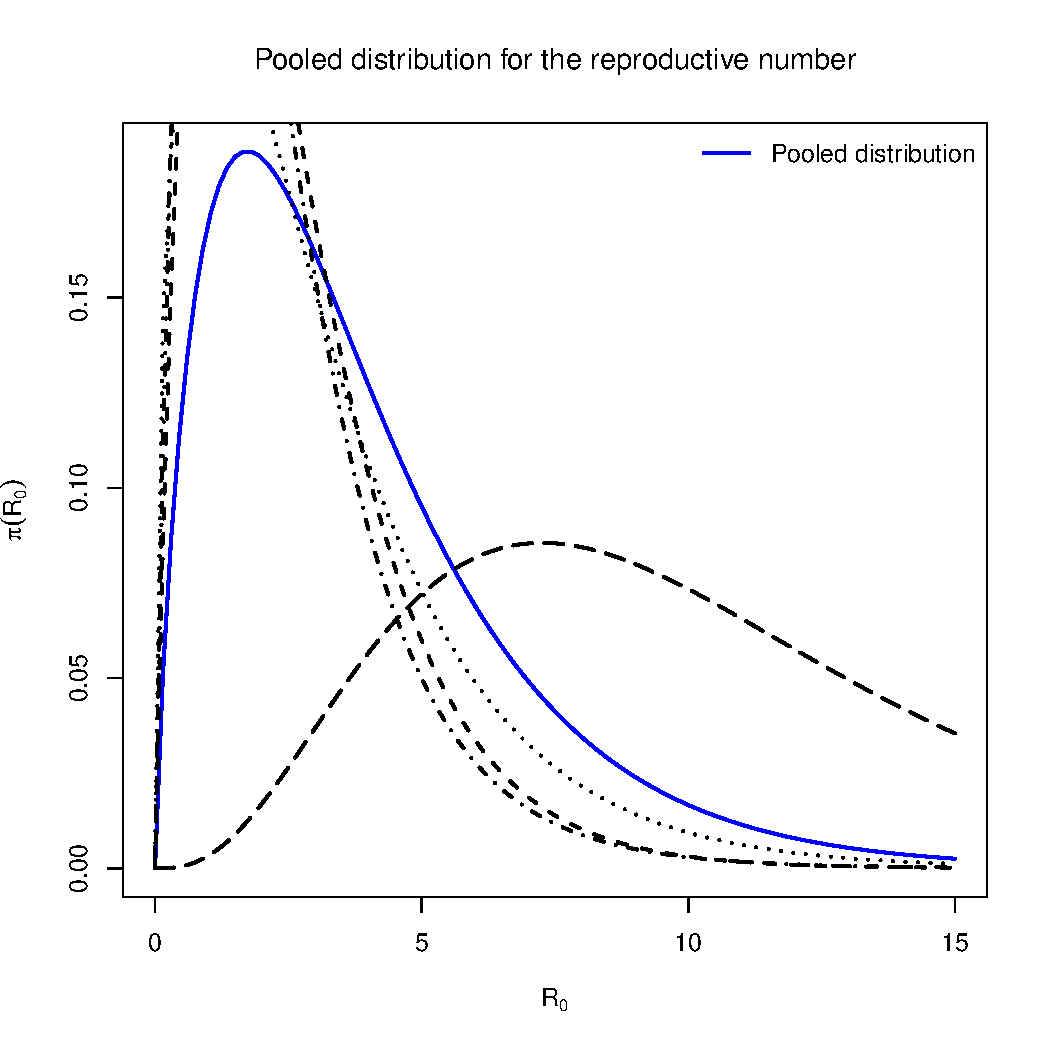
\includegraphics[scale=0.35]{figures/minKL_R0.pdf}}
\hfill
\caption{\textbf{Distributions for $R_0$}.
In panel A we present the `induce-then-pool'' and ``pool-then-induce'' distributions using equal weights ($\alpha_i = 1/K \:, \forall i$).
Panel B shows the pooled distribution for $R_0$ that minimises KL divergence with the ``induce-then-pool'' distribution, i.e., that minimises discrepancy in transformed space.
}
\label{fig:abstractFigure}
\end{figure}
\end{document}          
